\documentclass[11pt,a4paper]{article}

\usepackage[polish]{babel}
\usepackage[utf8]{inputenc}
\usepackage{polski}
\usepackage[T1]{fontenc}
\usepackage{indentfirst}
\usepackage{wrapfig}    % for wrapping figures, tables

\frenchspacing

\usepackage{amsmath}
%\usepackage{bm}
\usepackage{gensymb}
%\usepackage{hepnames}
\usepackage{epsfig}
\usepackage{graphics}
\usepackage[shortlabels]{enumitem}
%\usepackage{xspace}
%\xspaceaddexceptions{[]\{\}}

%
%
%fixpagesize
\pagestyle{empty}
\addtolength{\textwidth}{6cm}
\addtolength{\textheight}{4cm}
\addtolength{\evensidemargin}{-3cm}
\addtolength{\oddsidemargin}{-3cm}
\addtolength{\topmargin}{-2cm}
\parindent=0cm


%
%
%small distance in list/item/enum for enumitem package
\setlist[itemize,enumerate]{topsep=0em}
\setlist{noitemsep}

%print zadanie #
\newcounter{zadanie}\newcommand{\zadanie}[1][]{\addtocounter{zadanie}{1} ~\\  {\bf \emph{Zadanie \arabic{zadanie} #1 }} \\}
\newcounter{zaddom}\newcommand{\zaddom}[1][]{\addtocounter{zaddom}{1} ~\\  {\bf \emph{Zadanie domowe \arabic{zaddom} #1 }} \\}
%\renewcommand{\zadanie}[1][]{\pagebreak  ~\\  {\bf \emph{Zadanie }} \\} \addtolength{\topmargin}{-2cm}


%%%%%%%%%%%%%%%%%%%%%%%%%%%%%%%%%%%%%%%%%%%%%%%%%%%%%%
\begin{document}           % End of preamble and beginning of text.
\vspace*{-1.8cm}

\begin{centering}
\bf{\Large{Termodynamika z elementami fizyki statystycznej}}\\
Ćwiczenia 2 (6 marca 2024)\\[1mm]
własności cieplne cd. \\
\end{centering}

%%%%%%%%%%%%%%%%%%%%%%%%%%%%%%%%%%%%%%%%%%%%%%%%%%%%%%
\zadanie
Przy długości fali $\lambda = 0.7\,\mu$m porównano natężenie promieniowania dwóch,
doskonale czarnych, źródeł promieniowania o różnych temperaturach.
Temperatura pierwszego ciała wynosi $T_1 = 1068 \degree$C (topnienie złota). 
Znaleźć temperaturę drugiego ciała $T_2$, jeśli stosunek natężeń promieniowania 
wynosił $I_\lambda (T_2)/I_\lambda (T_1) = 10$.
Przyjmij $hc = 1.24$~eV$\mu$m

\vskip 10pt
\textbf{Rozwiązanie:}\\
Z prawa promieniowanie Plancka wiemy, że natężenie promieniowania w danej długości fali wynosi:

\begin{equation}
I_\lambda(T) = \frac{2 \pi h c^2}{\lambda^5} \frac{1}{\exp\left(\frac{h c}{\lambda k_B T}\right)-1}.
\label{planck}
\end{equation}

Zatem stosunek natężeń podany w zadaniu możemy zapisać jako:

\begin{equation}
  R=\frac{I_\lambda(T_2)}{I_\lambda(T_1)} =
  \frac{\exp\left(\frac{h c}{\lambda k_B T_1}\right)-1}{\exp\left(\frac{h c}{\lambda k_B T_2}\right)-1},\label{fraction}
\end{equation}

gdzie chwilowo zamiast wartości liczbowej stosunku natężeń wstawiliśmy zmienną $R$. W zakresie temperatur rozważanym w naszym zadaniu wartość funkcji $\exp$ w równaniu \eqref{fraction} jest wystarczająco duża, aby zaniedbać $-1$ w liczniku i mianowniku. Równanie upraszcza się do:

\begin{equation}
R = \exp\left(\frac{h c}{\lambda k_B}\left( \frac{1}{T_1}-\frac{1}{T_2}\right)\right).
\end{equation}

Rozwiązując ze względu na $T_2$ dostajemy:
\begin{align}
&\frac{1}{T_1}-\frac{1}{T_2} = \frac{\lambda k_B}{h c} \log(R)\\
  &T_2 = \frac{1}{\frac{1}{T_1} - \frac{\lambda k_B}{h c} \log(R)} =
  \frac{T_1}{1-\frac{\lambda k_B T_1}{h c} \log(R)} = 1578 K = 1305 ^\circ C.
\end{align}

Rozwiązując równanie \eqref{fraction} bez przybliżeń otrzymamy taki sam wynik:
\begin{equation}
T_2 = \frac{hc}{\lambda k_{B}} \ln^{-1}\left[\frac{\exp\left(\frac{h c}{\lambda k_B T_1}\right)-1}{R}+1 \right] = 1578 K
\end{equation}

%%%%%%%%%%%%%%%%%%%%%%%%%%%%%%%%%%%%%%%%%%%%
\newpage
%%%%%%%%%%%%%%%%%%%%%%%%%%%%%%%%%%%%%%%%%%%%

\zadanie [(Pirometr dwubarwny)]
Wyznaczyć temperaturę ciała świecącego wiedząc, że stosunek natężeń promieniowania dla długości fal
$\lambda_1=550$\,nm i $\lambda_2=700$\,nm wynosi $R=I_{\lambda_2}(T)/I_{\lambda_1}(T) =1.286$.
Przyjąć $T \sim 10^{3}$~K.\\

\vskip 10pt
\textbf{Rozwiązanie:}\\
Znowu korzystamy z prawa Plancka (rów. \eqref{planck}), tym razem przy ustalonej temperaturze:

\begin{equation}
  R = \frac{I_{\lambda_2}(T)}{I_{\lambda_1}(T)} =
  \frac{\lambda_1^5}{\lambda_2^5}
  \frac{\exp\left(\frac{h c}{\lambda_1 k_B T}\right)-1}{\exp\left(\frac{h c}{\lambda_2 k_B T}\right)-1}. \label{planck2}
\end{equation}

Wartości funkcji $\exp$ w równaniu \eqref{planck2} znów są na tyle duże, że możemy zaniedbać
wyrazy $-1$ w liczniku i mianowniku. Otrzymujemy proste równanie:

\begin{equation}
R = \frac{\lambda_1^5}{\lambda_2^5} \exp\left(\frac{h c}{T k_B}\left( \frac{1}{\lambda_1}-\frac{1}{\lambda_2}\right)\right).
\end{equation}

Bierzemy logarytm i upraszczamy równanie, aby dostać:

\begin{align}
&\log(R) = 5 \log\left(\frac{\lambda_1}{\lambda_2}\right) + \frac{h c}{T k_B}\left( \frac{1}{\lambda_1}-\frac{1}{\lambda_2}\right),\\
  &T = \frac{\frac{h c}{k_B}\left( \frac{1}{\lambda_1}-
    \frac{1}{\lambda_2}\right)}{\log(R)-5 \log\left(\frac{\lambda_1}{\lambda_2}\right)} =  3845K
\end{align}

Wynik możemy porównać z rozwiązaniem numerycznym $T \approx 3858K$ w serwisie Wolphram Alpha
(komenda solve przekracza czas obliczeń na darmowym koncie):
\begin{verbatim}
plot  (exp(26154/x) - 1)/(exp(20550/x) - 1)-4.29 from 3855 to 3860
\end{verbatim}

%%%%%%%%%%%%%%%%%%%%%%%%%%%%%%%%%%%%%%%%%%%%
\newpage
%%%%%%%%%%%%%%%%%%%%%%%%%%%%%%%%%%%%%%%%%%%%
\zadanie

Wyznaczyć temperaturę Ziemi zakładając, że znajduje się ona w równowadze radiacyjnej ze
Słońcem. Temperatura Słońca wynosi $T_\odot = 5800$~K, a promień $R_\odot = 7 \cdot 10^8$~m.
Odległość między Ziemią a Słońcem wynosi $D = 1.5 \cdot 10^{11}$~m. 
Przyjąć, że temperatura na powierzchni Ziemi jest stała podczas całego cyklu dobowego.
Obliczenia należy wykonać w dwóch wariantach:\\
\begin{enumerate}[a)]
        \item Ziemia jest ciałem doskonale czarnym i nie posiada atmosfery.
        \item Ziemia jest ciałem doskonale czarnym i posiada atmosferę w postaci sfery o promieniu niewiele większym od promienia Ziemi. 
        W modelu tym $\alpha=40\%$ promieniowania pochodzącego ze Słońca odbija się od górnych warstw atmosfery, zaś pozostałe $60\%$ 
        przenika przez atmosferę i zostaje pochłonięte przez Ziemię. Atmosfera pochłania całe promieniowanie wyemitowane przez Ziemię
  (promieniowanie Ziemi ma inny zakres długości fal niż promieniowanie Słońca). Atmosfera jest w równowadze tylko z Ziemią, 
  ponieważ nie absorbuje promieniowania słonecznego.
\end{enumerate}
%Otrzymany wynik należy porównać z rzeczywistą średnią temperaturą
%Ziemi równą $15^\circ C$.

\vskip 10pt
\textbf{Rozwiązanie:}\\
Moc wyemitowana przez Słońce, wynosi
$P_\odot = 4\pi R_\odot^2 \sigma T_\odot^4 $. Moc na jednostkę powierzchni docierająca
do Ziemi wynosi 
$$
{\cal I}_{in} = \frac{P_\odot}{ 4\pi D^2} =  \sigma T_\odot^4 \left(\frac{R_\odot}{D}\right)^2
$$
Moc absorbowana przez Ziemię (w przypadku bez atmosfery)
$$
P_{in} =  \sigma T_\odot^4 \left(\frac{R_\odot}{D}\right)^2 \pi R_z ^2,
$$
gdzie $R_z$ jest promieniem Ziemi.
Moc emitowana przez Ziemię:
$$
P_{out} = 4\pi R_z^2 \sigma T_z^4.
$$
W równowadze $P_{in}=P_{out}$ więc otrzymujemy
$$
T_z = T_\odot \sqrt{\frac{R_\odot}{ D}}\frac{1}{4^{1/4}} \approx 280 K \approx 7^\circ C.
$$

W przypadku z atmosferą 
Ziemia pochłania część promieniowania pochodzącego ze Słońca oraz część promieniowania 
pochodzącego od atmosfery 
$$
P_{in} = (1-\alpha)\sigma T_\odot^4 \left(\frac{R_\odot}{D}\right)^2 \pi R_z ^2
+ \frac{1}{2} P_{atm},
$$
natomiast emituje
$$
P_{out} = 4\pi R_z^2 \sigma T_z^4.
$$
Otrzymujemy więc
$$
4\pi R_z^2 \sigma T_z^4 = (1-\alpha)\sigma T_\odot^4 \left(\frac{R_\odot}{D}\right)^2 \pi R_z ^2
+ \frac{1}{2} P_{atm}
$$

Atmosfera pochłania całe promieniowanie wyemitowane przez  Ziemię  
$$
P_{atm} =  4\pi R_z^2 \sigma T_z^4.
$$
Podstawiając do poprzedniego równania otrzymujemy
$$
4   T_z^4 = (1-\alpha)T_\odot^4 \left(\frac{R_\odot}{D}\right)^2  
+ 2  T_z^4 
$$
otrzymujemy
$$
T_z = T_\odot \sqrt{\frac{R_\odot}{ D}} \left[\frac{1-\alpha}{2}\right]^{1/4}
$$
W przypadku $\alpha=0.4$ otrzymujemy $T_z \approx 293.23 K \approx 20^\circ C$.


%%%%%%%%%%%%%%%%%%%%%%%%%%%%%%%%%%%%%%%%%%%%
\newpage
%%%%%%%%%%%%%%%%%%%%%%%%%%%%%%%%%%%%%%%%%%%%

\zadanie [(Termos próżniowy I)]
Dane są dwie nieskończone doskonale czarne płaszczyzny o temperaturach $T_1=300\,$K i $T_2=4$\,K.
Obliczyć strumień energii (czyli moc na jednostkę powierzchni)
przesyłaną między nimi. Rozważyć trzecią płaszczyznę (osłonę)
między nimi, która odbija $R$ = 95\% promieniowania. 
Obliczyć temperaturę osłony i strumień energii pomiędzy płaszczyznami.
Przyjmij $\sigma = 5.67\cdot 10^{-8}~\mathrm{W/m^{2}K^{4}}$

\vskip 10pt
\textbf{Rozwiązanie:}\\

\begin{wrapfigure}{r}{0.45\linewidth}\vspace{-0.1cm}
  \resizebox{\linewidth}{!}{\includegraphics[width=6cm]{termos.png}}
  \caption{Po lewej: dwie płyty; każda z nich emituje strumień promieniowania w całości absorbowany
    przez płytę po przeciwnej stronie.
    Po prawej: dodatkowa płyta, która odbija część promieniowania: $I_{1/2r}$.}
\end{wrapfigure}

W wariancie bez środkowej płyty sytuacja jest bardzo prosta. Każda płyta emituje promieniowanie
o strumieniu $\sigma T^4$, które absorbowane jest na przeciwnej płycie. Zatem strumień energii między płytami wynosi:
\begin{equation}
\Delta I = \sigma(T_1^4-T_2^4) = 459 \frac{W}{m^2}.
\end{equation}

Po dodaniu środkowej płyty na początek policzmy temperaturę $T_3$ analizując bilans energetyczny środkowej
płyty. \textbf{W każdą stronę} emituje ona promieniowanie o strumieniu $I_3 = (1-R)\sigma T_3^4$; absorbuje
za to $(1-R)\sigma (T_1^4 +T_2^4)$.
Dostajemy zatem równanie:

\begin{equation}
2(1-R) \sigma T_3^4 = (1-R) \sigma (T_1^4+T_2^4), \quad T_3 = \sqrt[4]{\frac{T_1^4+T_2^4}{2}}= 252 K.
\end{equation}

Co ciekawe wynik ten nie zależy od $R$.

Możemy teraz policzyć strumień energii między płytami. Między lewą a środkową płytą mamy:

\begin{equation}
  \Delta I_1 = \sigma (  T_1^4- R T_1^4 - (1-R)T_3^4) = \sigma (1-R) (T_1^4-T_3^4) =
  \sigma(1-R) \frac{(T_1^4-T_2^4)}{2} = 11.5 \frac{W}{m^2}.
\end{equation}

Dla sprawdzenia policzmy także strumień między środkową a prawą płytą:

\begin{equation}
  \Delta I_2 = \sigma (  -T_2^4 + R T_2^4 + (1-R)T_3^4) =
  \sigma (1-R) (T_3^4-T_2^4) = \sigma(1-R) \frac{(T_1^4-T_2^4)}{2}.
\end{equation}

Zgodnie z oczekiwaniami (jesteśmy w stanie równowagi, więc środkowa płyta nie magazynuje energii)
otrzymaliśmy dokładnie ten sam wynik po obu stronach środkowej płyty. Zauważmy, że gdy środkowa płyta
jest doskonale czarna ($R=0$), strumień energii spada dwukrotnie.

%%%%%%%%%%%%%%%%%%%%%%%%%%%%%%%%%%%%%%%%%%%%
\newpage
%%%%%%%%%%%%%%%%%%%%%%%%%%%%%%%%%%%%%%%%%%%%
\zadanie [(Termos próżniowy II)]
Dwie równoległe, duże, doskonale czarne płyty umieszczone są w próżni i mają temperatury $T_1$ i $T_2$.
Między te płyty wstawiamy równolegle do nich $n$ dużych, cienkich, doskonale czarnych płyt.
Jaka jest temperatura $i$-tej płyty? 
Ile razy, w wyniku wstawienia płytek, zmniejszy się strumień energii pomiędzy płaszczyznami? 

\resizebox{0.93\linewidth}{!}{\includegraphics[width=6cm]{termos_2_page1.png}}

\resizebox{\linewidth}{!}{\includegraphics[width=6cm]{termos_2_page2.png}}

\resizebox{\linewidth}{!}{\includegraphics[width=6cm]{termos_2_page3.png}}

%%%%%%%%%%%%%%%%%%%%%%%%%%%%%%%%%%%%%%%%%%%%
\newpage
%%%%%%%%%%%%%%%%%%%%%%%%%%%%%%%%%%%%%%%%%%%%

\zadanie
Korzystając z prawa promieniowania Plancka wykaż prawo Stefana-Boltzmanna:  $I(T) = \sigma T^4$.
Całkę jaka pojawi się w obliczeniach oznacz jako $\sigma$ i nie wykonuj jej explicite.


\vskip 10pt
\textbf{Rozwiązanie:}\\
Całkowite natężenie promieniowania otrzymamy poprzez całkę po długościach fali z równania \eqref{planck}:

\begin{equation}
  I(T) = \int_0^\infty I_\lambda(T) d\lambda =
  \int_0^\infty \frac{2 \pi h c^2}{\lambda^5} \frac{1}{\exp\left(\frac{h c}{\lambda k_B T}\right)-1} d\lambda. \label{integral}
\end{equation}

Nie chcemy policzyć dokładnej wartości całki \eqref{integral}. Zamiast tego możemy wyciągnąć poza
całkę zależność od temperatury, a całkę zostawić jako współczynnik stałej fizycznej, którą można
zmierzyć doświadczalnie. W tym celu wprowadzamy bezwymiarową zmienną całkowania:

\begin{equation}
x = \frac{h c}{\lambda k_B T}, \quad \lambda = \frac{h c}{x k_B T},\quad d\lambda = - \frac{h c dx}{k_B T x^2}.
\end{equation}

Po zamianie zmiennych natężenie promieniowania przyjmuje postać:
\begin{equation}
  I(T) = 2 \pi h c^2 \int_0^\infty \left(\frac{xk_B T}{hc}\right)^5 \frac{1}{\exp(x)-1}
  \frac{h c dx}{k_B T x^2} =
  2 \pi \frac{k_B^4 T^4}{h^3 c^2} \int_0^\infty \frac{x^3 dx}{\exp(x)-1} = \sigma T^4.
\end{equation}
Otrzymaliśmy prawo Stefana-Boltzmanna ze stałą $\sigma = 2 \pi \frac{k_B^4}{ h^3 c^2} \int_0^\infty \frac{x^3 dx}{\exp(x)-1}$.

\pagebreak
\begin{centering}
\bf{ Zadania domowe }\\[1mm]
\end{centering}
\vspace{1mm}

\zaddom
Zale"rno"s"c ci"snienia r"ownowagi fazy ciek"lej i lotnej opisuje 
w przybli"reniu wz"or: $ p \,=\, A e^{-\alpha/T} $.\\
Dla wody: $p_3 = 612\,$Pa, $T_3 = 273.16\,$K, 
$p_{\rm wrzenia} = 1.013\cdot 10^5\,$Pa, 
$T_{\rm wrzenia} = 373.2\,$K.\\ 
Wyznacz sta"le $A$ i $\alpha$.
Oblicz w jakiej temperaturze woda wrze na wysoko"sciach:
\begin{enumerate}[a)] 
\item 2500\,m -- Rysy ($p = 0.75\,$bar)
\item 4800\,m -- Mont Blanc ($p = 0.55\,$bar)
\item 8850\,m -- Mont Everest ($p = 0.33\,$bar).
\end{enumerate}
Przy jakim ci"snieniu woda wrze w temperaturze $20^\circ$C\,? $-3^\circ$C\,?

\zaddom
Do budowy termoregulator"ow, ogranicznik"ow temperatury i tym
podobnych urz"adze"n stosuje si"e cz"esto urz"adzenie zwane bimetalem.
Jest to pasek z"lo"rony z dw"och spojonych ze sob"a warstw metali
o r"o"rnych wsp"o"lczynnikach rozszerzalno"sci.
Pasek taki przy ogrzewaniu b"edzie si"e wygina"l i mo"re
w ten spos"ob zamyka"c lub otwiera"c obw"od elektryczny.
Dany jest bimetal o grubo"sci $d$, z"lo"rony z metali
o wsp"o"lczynnikach rozszerzalno"sci liniowej $\alpha_1$ i $\alpha_2$
($\alpha_1 > \alpha_2$).
W temperaturze $T_0$ bimetal jest prosty.
Znajd"z promie"n krzywizny bimetalu po ogrzaniu go o $\Delta T$.
Wykonaj obliczenia dla: $\alpha_1=1.8\cdot 10^{-5}\,{\rm K}^{-1}$ (mosi"adz),
$\alpha_2=1.2\cdot 10^{-5}\,{\rm K}^{-1}$ (stal), grubo"s"c $d=1\,$mm,
d"lugo"s"c $l_0=5\,$cm, $\Delta T=100\,$K.

\zaddom
Op"or w"la"sciwy miedzi zależy od temperatury jak:
$ \rho(T) = 
  A \left(\frac{T}{T_0}\right) \tanh^3 \left(\frac{T}{T_0}\right);
  ~~ T_0 = 87\,\rm{K}. 
$
W temperaturze 290\,K miedziany czujnik ma op"or 10\,$\Omega$. 
\begin{enumerate}
\item Jaki op"or ma ten czujnik w temperaturze 700\,K? 
\item Jak zmieni si"e op"or dla temperatury 701\,K? Ile wynosi $\Delta R/R$? 
\item Jaki jest op"or w temperaturze 20\,K?
\item Jak zmieni si"e op"or dla temperatury 21\,K? Ile wynosi  $\Delta R/R$?
\end{enumerate}
Zadanie rozwiąż rachunkiem bezpośrednim oraz korzystając z odpowiednich rozwinięć.

\zaddom
Oszacuj całkowitą moc jaką wypromieniowujesz. Opisz przyjęte założenia i zastosowane przybliżenia. Oszacuj
wydatek energetyczny organizmu na utrzymanie temperatury ciała (różnicę pomiędzy mocą wypromieniowywaną
i otrzymywaną) jeżeli znajdujesz się w otoczeniu o temperaturze $20\degree$C.
Jakiej długości fali odpowiada maksimum rozkładu energii?

\zaddom
Sonda kosmiczna o kształcie kuli i doskonale czarnej powierzchni ma zbadać okolice Merkurego. Aby uniknąć
przegrzania sondy wyposażono ją w “ekran termiczny” - cienką osłonkę o kształcie półsfery zrobioną z metalu
o współczynniku odbicia r. Osłona założona jest bardzo blisko powierzcni sondy, ale nie styka się z nią. Sonda
zwrócona jest osłoniętą stroną do Słońca.
\begin{enumerate}
\item Znajdź wyrażenie na temperaturę sondy w funkcji jej odległości od Słońca i porównaj z temperaturą sondy
pozbawionej osłony
\item Dobierz współczynnik odbicia r tak aby w pobliżu Merkurego sonda miała temperaturę $T_{\rm sondy}= 300$\,K. 
Jaka jest wtedy temperatura osłony?
\end{enumerate}
Temperatura Słońca wynosi $T_\odot= 5800$\,K, promień Słońca $R_\odot = 7 \cdot 10^8$\,m, 
odległość Merkurego od Słońca $d = 5.8 \cdot 10^{10}$\,m. 
Zakładamy, że cała powierzchnia sondy ma tę samą temperaturę.

\end{document}
